\documentclass[12pt,tikz,border=5pt]{standalone}
\usetikzlibrary{mindmap,backgrounds}
\colorlet{col1}{teal}
\colorlet{col2}{olive}
\colorlet{col3}{orange}
\begin{document}
  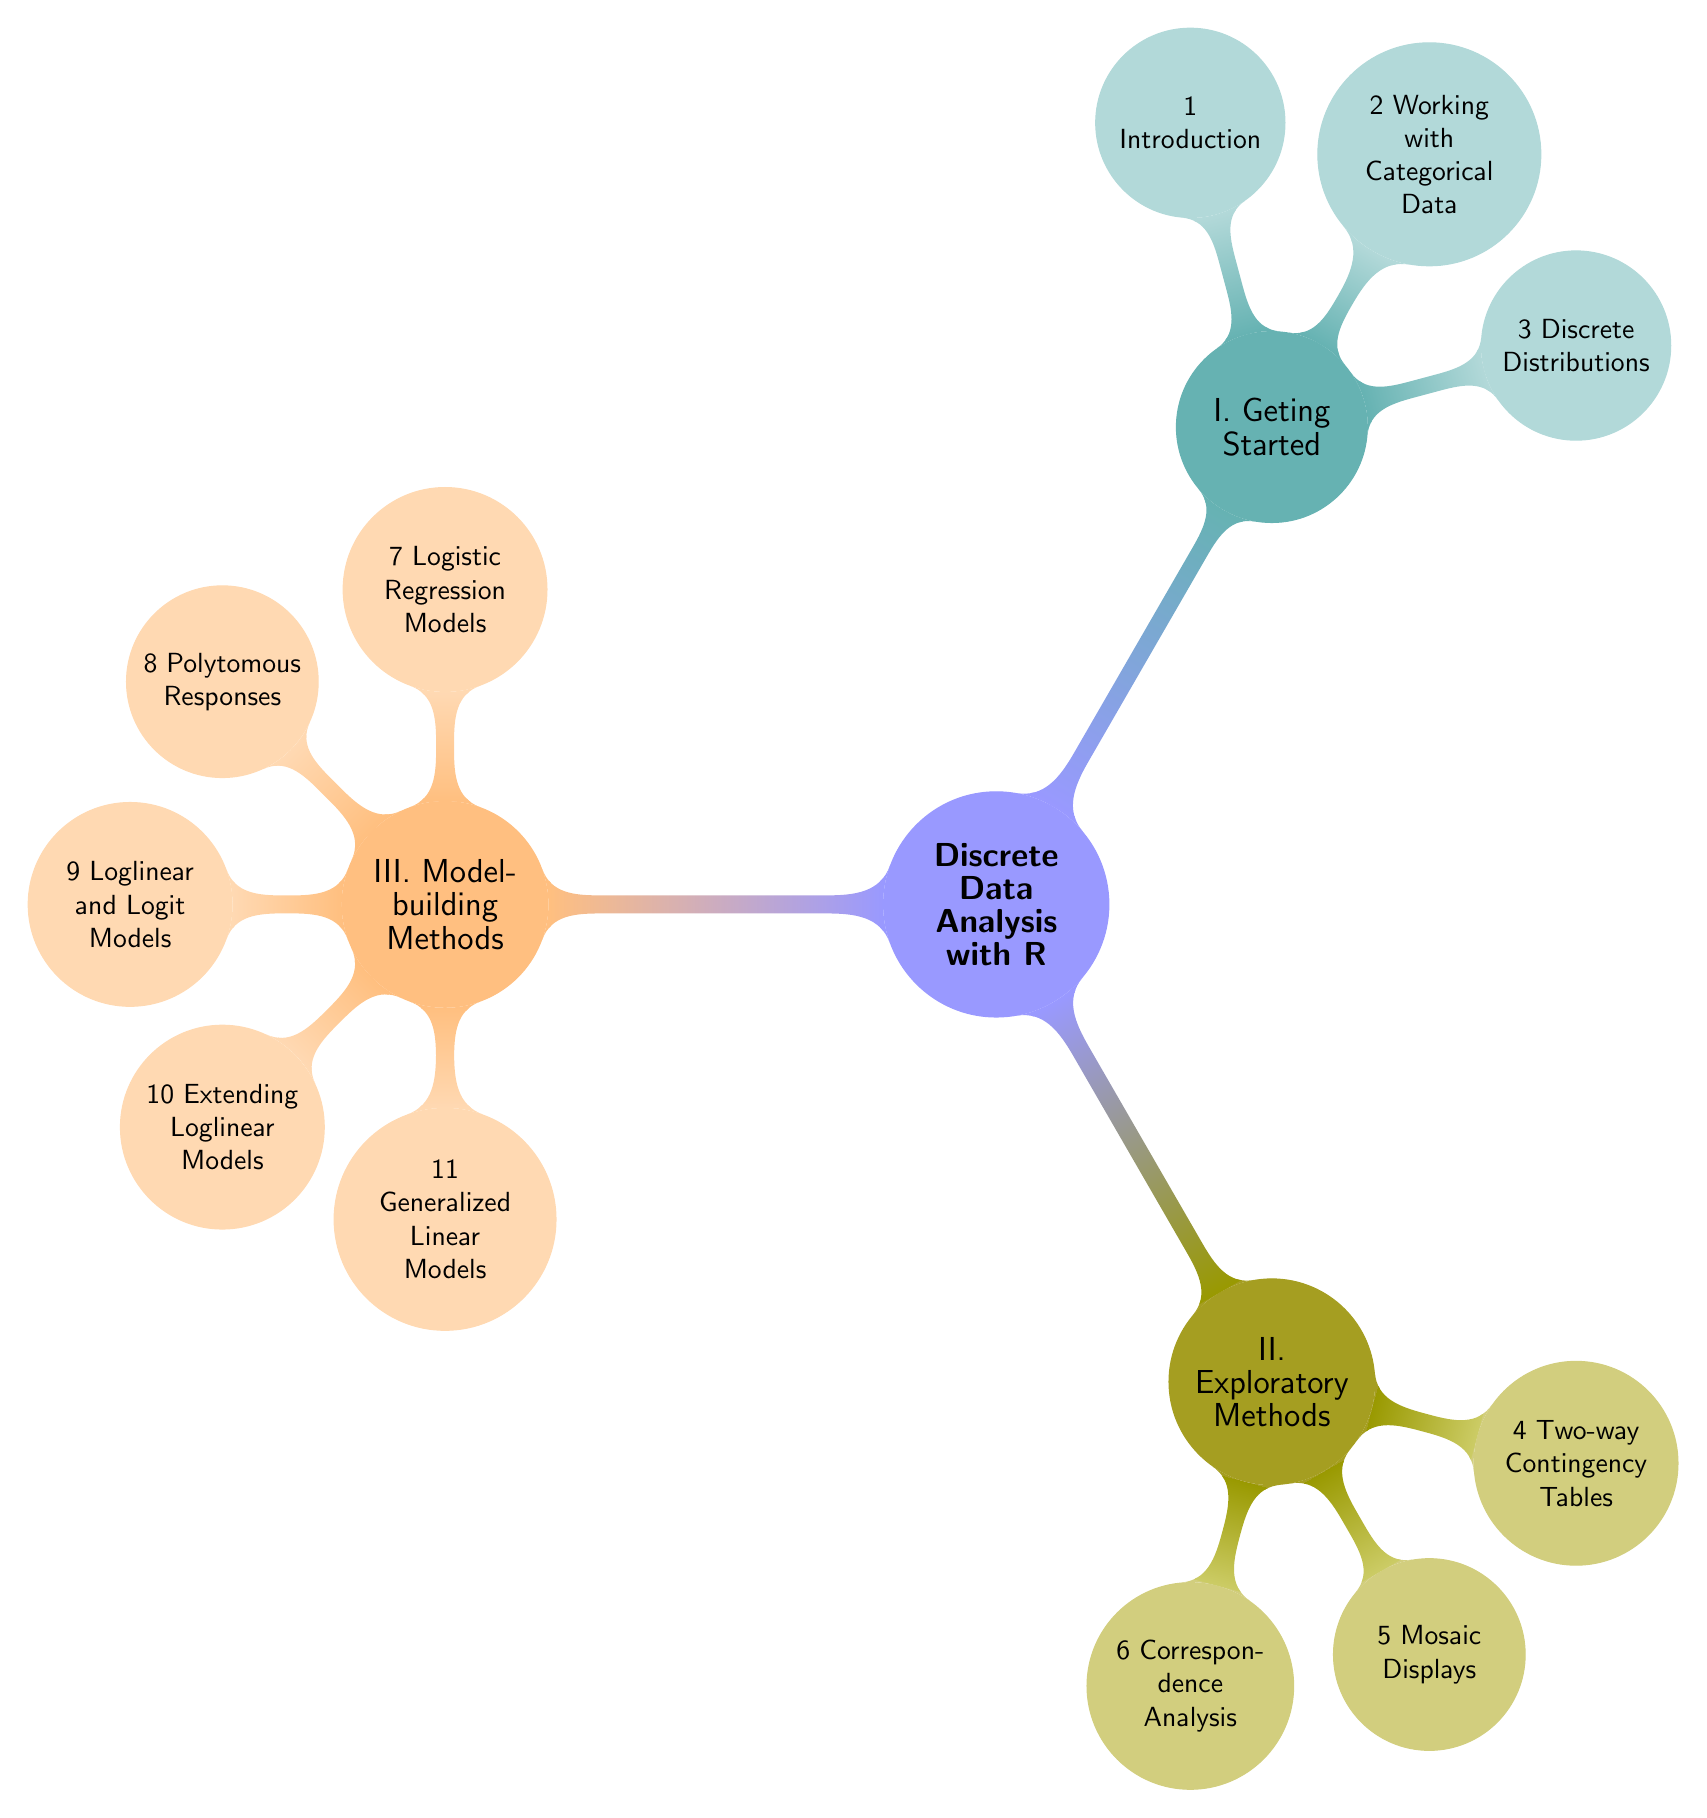
\begin{tikzpicture}[grow cyclic, text width=2cm, align=flush center, every node/.style=concept, concept color=blue!40,
    level 1/.style={level distance=7cm,sibling angle=120},
    level 2/.style={level distance=4cm,sibling angle=45}]
    \sffamily

    \node{\textbf{\large Discrete Data Analysis with R}} [clockwise from=60]  % root node
    child [concept color=col1!60] { node {\large I. Geting Started}
      [clockwise from=105]
      child [concept color=col1!30] { node (ch1) {1 Introduction}}
      child [concept color=col1!30] { node (ch2) {2 Working with Categorical Data}}
      child [concept color=col1!30] { node (ch3) {3 Discrete Distributions}}
    }
    child [concept color=col2!80] { node [concept] {\large II. \\ Exploratory  Methods}  [clockwise from=60]
      [clockwise from=-15]
      child [concept color=col2!40] { node (ch4) {4 Two-way Contingency Tables}}
      child [concept color=col2!40] { node (ch5) {5 Mosaic Displays}}
      child [concept color=col2!40] { node (ch6) {6 Correspondence Analysis}}
    }
    child [concept color=col3!50] { node {\large III. Model-building Methods}  [counterclockwise from=90]
      child [concept color=col3!30] { node (ch7) {7 Logistic Regression Models}}
      child [concept color=col3!30] { node (ch8) {8  Polytomous Responses}}
      child [concept color=col3!30] { node (ch9) {9 Loglinear and Logit Models}}
      child [concept color=col3!30] { node (ch10) {10 Extending Loglinear Models}}
      child [concept color=col3!30] { node (ch11) {11 Generalized Linear Models}}
    };
%    \begin{scope}[on background layer]
%%      \path (ch5) to[circle connection bar switch color=from (col2!40) to (col3!30)] (ch9);
% %     \path (ch3) to[circle connection bar switch color=from (col1!30) to (col3!30)] (ch11);
%      \draw [concept connection] (ch5) edge (ch9);
%      \draw [concept connection] (ch5) edge (ch7);
%      \draw [concept connection] (ch3) edge (ch11);
%      \draw [concept connection] (ch4) edge (ch5);
%      \draw [concept connection] (ch5) edge (ch6);
%      \draw [concept connection] (ch7) edge (ch8);
%      \draw [concept connection] (ch9) edge (ch10);
%
%    \end{scope}
  \end{tikzpicture}
\end{document}